
\begin{figure}[htbp]
    \centering
  	\begin{subfigure}[t]{\floatwidth}
  	    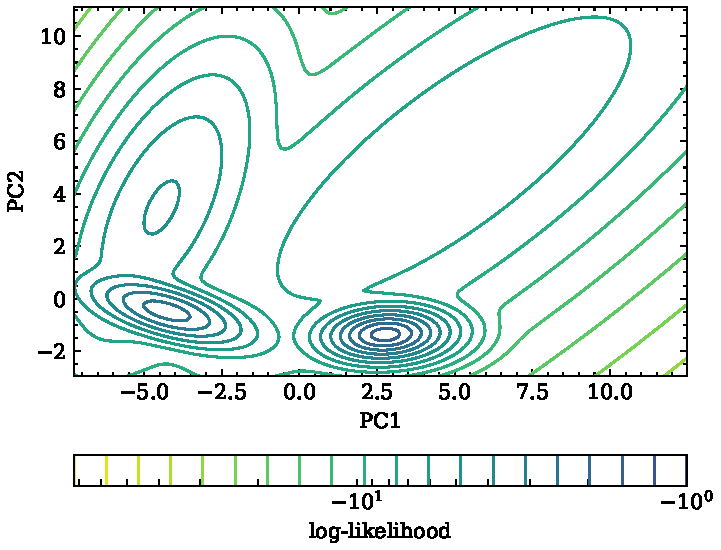
\includegraphics[width=\textwidth]{5Results/figs/embeddings/gmm_density.pdf}
  	    \caption{log-likelihood as predicted by GMM}
  	\end{subfigure}
    \Caption{Embedding of EEG}{
	2-channel segments of duration 10 (s), randomly sampled from the training set, are embedded in the GP parameter space. A GMM fit with expectation-maximization provides an approximate density estimation. Higher values are more likely to be generated by the GMM.
    \protect \NS[inline]{fix class labels in legend, remove redundant axis label}}
    \label{fig:5results:embeddings}
\end{figure}

